\chapter{Measurement of the inclusive $t\bar{t}+\gamma$ cross-section}\label{chap-crosssection}

\begin{figure}
\begin{center}
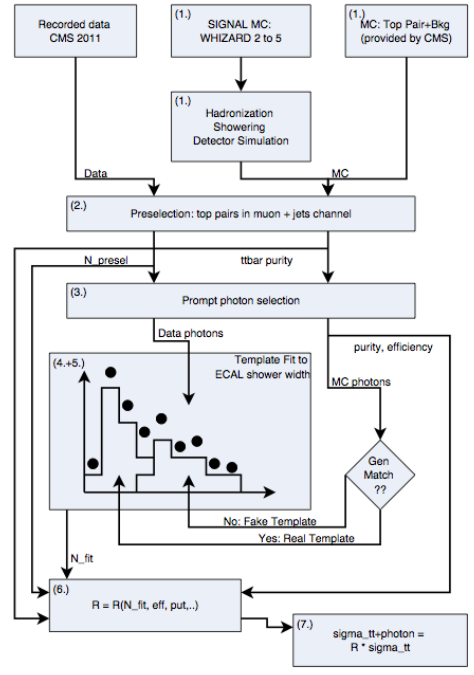
\includegraphics[width=0.75\textwidth]{Figures/AnalysisFlowChart.png}
\end{center}
\caption{Flow chart showing each stage of the analysis. The box numbers represent the outlined
analysis steps.}
\label{fig-AnalysisFlowChart}
\end{figure}

\section{Measurement of the cross-section ratio $R = \sigma_{t\bar{t}+\gamma}/\sigma_{t\bar{t}}$}

A common form of cross-section calculation for a ``counting'' analysis can be written as

\begin{equation} \label{eqn-CountingXsect}
\sigma = \frac{N_{signal}}{\lumi \epsilon A}
\end{equation}

where $N_{signal}$ is the number of signal events found in data passing the full event selection requirements, $\lumi$ is the integrated luminosity of the data, $A$ is the signal acceptance, defined as the fraction of signal events that fall into the region of phase-space that is chosen for our event selection, and $\epsilon$ is the efficiency of correctly selecting a signal event (the fraction of signal events passing event selection after acceptance cuts are implemented). The number of signal events, $N_{signal}$, must be modified to account for the presence of background events in our data, and thus becomes the number of observed events minus the number of background events, $N_{observed} - N_{background}$, where the number of background events is estimated in a different manner. 

Due to the nature of the analysis, event selection is performed in two separate steps (see Section \ref{chap-EventSelection}); di-leptonic top pair selection and photon selection. This feature changes the way in which we must compute the cross-section in Equation \ref{eqn-CountingXsect}. The changed cross-section is written as

\begin{equation}
\sigma_{t\bar{t}+\gamma} = \frac{N_{signal}}{\lumi \epsilon_{top} A_{top} \epsilon_{\gamma} A_{\gamma}}
\end{equation}

where $\epsilon_{top}$ and $A_{top}$ are the efficiency and acceptance of top selection for our signal top pair events. Thus, $\epsilon_{\gamma}$ and $A_{\gamma}$ are the efficiency and acceptance of the photon selection, introduced after the top quark pair event selection. Here we consider our signal as a top quark pair, decaying to leptons and b-jets, plus a prompt radiatied photon as our signal. We take the number of observed, $N_{signal}$, as the number of events counted from data after top pair and photon selections have been applied.

Within this analysis, we measure the fiducial cross-section by calculating the cross-section of all events that fall within our chosen kinematic selection requirements introduced by the top and photon selection parameters. In reality, we calculate the fiducial cross-section, $t\bar{t}+\gamma$, by diving by the acceptance as such:

\begin{equation}
\sigma_{t\bar{t}+\gamma}^{fid.} = \frac{N_{t\bar{t}+\gamma}}{\epsilon \cdot \lumi}, \quad \sigma_{t\bar{t}+\gamma} = \frac{N_{t\bar{t}+\gamma}}{A \cdot \epsilon \cdot \lumi} = \frac{\sigma_{t\bar{t}+\gamma}^{fid.}}{A}
\end{equation}

In order to simplify the calculation, we are able to take the ratio of the fiducial $t\bar{t}+\gamma$ cross-section to the inclusive $t\bar{t}$ cross-section, as previously measured by the CMS experiment \cite{ttbarXsectiondilepton}. In doing this, we simplfy the treatment of systematic uncertainties and cancel shared terms from each measurement, such as luminosity. The new ratio is calculated using the following equation

\begin{equation}
R = \frac{\sigma_{t\bar{t}+\gamma}^{fid.}}{\sigma_{t\bar{t}}^{incl.}} = \frac{\sigma_{t\bar{t}+\gamma}^{fid.}}{1}\cdot\frac{1}{\sigma_{t\bar{t}}^{incl.}} = \frac{N_{t\bar{t}+\gamma}^{signal}}{\epsilon_{t\bar{t}+\gamma}^{top+pho.}} \cdot \frac{(\epsilon \cdot A)_{t\bar{t}}^{top}}{N_{t\bar{t}}}
\end{equation}

We now introduce a second term into the cross-section calculation which includes three new variables that stem from the $t\bar{t}$ inclusive cross-section: where $\epsilon_{t\bar{t}}^{top}$ and $A_{t\bar{t}}^{top}$ are the efficiency and acceptance of the $t\bar{t}$ process, $N_{t\bar{t}}$ is the number of top pair events passing the full top selection prior to the photon selection, and $\epsilon_{t\bar{t}+\gamma}^{top+pho.}$the efficiency of finding $t\bar{t}+\gamma$ events after top and photon selection. We define the efficiency for $t\bar{t}+\gamma$ with top pair and photon selection as

\begin{equation}
\epsilon_{t\bar{t}+\gamma}^{top+pho.} = \frac{N_{t\bar{t}+\gamma}^{pho.}}{N_{t\bar{t}+\gamma}^{gen. fid.}}
\end{equation}


where $N_{t\bar{t}+\gamma}^{pho.}$ is the number of $t\bar{t}+\gamma$ events passing photon selection, including migration into the fiducial region, and $N_{t\bar{t}+\gamma}^{gen. fid.}$ is the number of $t\bar{t}+\gamma$ events at generator level passing fiducial cuts, where fiducial cuts include both top and photon selection requirements. The efficiencies for both top pair selection and top pair with a photon selection is very similar due to the ordering of the event selection - the selection of leptons, jets, b-jets, and MET are the same in each scenario. As the acceptance calculation depends on individual samples generator cuts and even selection, we must calculate this variable separately for each stage of the selection process. By taking the ratio of each cross-section we cancel out the luminosity parameter.

The prominent feature of this analysis is the addition of a radiated photon from one of the decay products of a dileptonic $t\bar{t}$ decay. In order to correctly measure the number of signal $t\bar{t}+\gamma$ events we must make sure that we have correctly identified our signal events. Even though an object may pass the full photon ID selection requirements, it may not be our signal photon. Electrons and jets are likely to pass photon ID selection and be recorded as real signal photons, thus we must remove these ``fakes" from our signal events.

For jets that pass the photon ID requirements and are thus misidentified, we must note that they do not contain a genuine photon. Electrons that have been misidentified as photons are more difficult to remove as they hold the same properties as a photon, including isolated electromagnetic shower etc. Electrons differ from our signal photons because of the addition of a charged track pointing in the direction of the energy deposit. As a result, we treat each source of ``fakes" in a different manner, described in Section \ref{sec-PhotonPurityEstimation}.



% \section{Number of top pair events}

% \cite{PhysRevD.89.092005}

\section{Photon Purity Estimation} \label{sec-PhotonPurityEstimation}

We define the photon purity, $\pi$, as the number of photons that are prompt and pass the photon ID selection over the total number of photon candidates. Prompt photons are created in the hard-scattering process and are emitted from the high-$p_T$ hard-scattering particles. The main sources of non-prompt photons comes from charged particles interacting with the detector material and from quark hadronisation, and are generally not isolated and have a low $p_T$. We also obtain a source of photons from $\pi^0$ decays, whereby two very collinear photons are produced. A graphical representation of the definitions of signal and background for the $t\bar{t}+\gamma$ process can be seen in Figure \ref{fig-signalphotonplot}

\begin{figure} 
\begin{center}
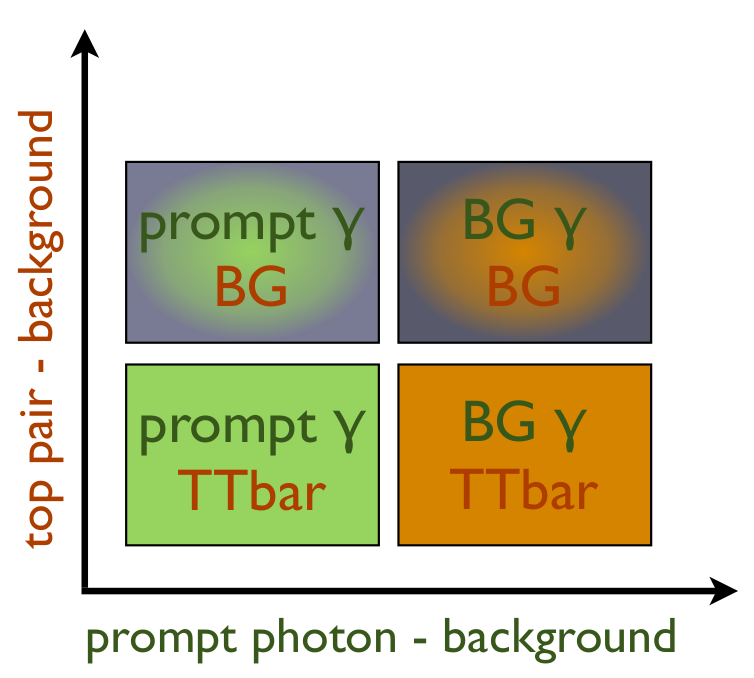
\includegraphics[scale=0.33]{Figures/SignalPhotonPlot.png}
\end{center}
\caption{Graphic representation of the signal and background definitions \cite{MishaThesis}.}
\label{fig-signalphotonplot}
\end{figure} 

One method to find the photon purity is through simulation, where we have access to information of all the particles simulated by the MC event generator. We match reconstructed photons to generator photons by using information of their mother particles in order to determine the origin of the photons. From this we can divide our events into three categories based on the event generator matching to a reconstructed photon. 

\begin{itemize}
	\item Signal: reconstructed photon is matched to a generated photon
	\item Misidentified electron: reconstructed photon is matched to a generated electron
	\item Misidentified jet: photon is not matched to either a generated photon or electron
\end{itemize}

In order to find if our photon is prompt (signal), we use our matching process to find a generator-level photon that matches its properties. We use the transverse momentum along with the $\eta$ and $\phi$ coordinates of the reconstructed and generator-level photon to implement a $p_T$ and $\Delta R$ requirement on the matching process. Events are iterated over in the order in which they were created by the generator, and if we find the $\Delta R$ between the reconstructed photon and generated photon is \textbf{less than 0.2} and $|p^{reco}_T - p^{gen}_T|/p^{gen}_T$ is \textbf{less than 1.0} then we consider it a match and stop the iteration process. The parentage of the matched photon is then inspected to verify its origin, such that if it descends from a quark, gluon, charged lepton, or boson then we determine it to be prompt. We must, however, also verify that the photon is isolated. A photon maybe produced in the hard-scattering process, however we may observe hadronisation and showering in close by, such that our signal photon will not be isolated. In order to ensure that these photons are not lost to the nearby non-signal activity, we must introduce additional selection cuts to differentiate between our prompt signal photons and non-isolated photons.  

\begin{itemize}
	\item $\left(p_T^{reco} - p_T^{gen}\right)/p_T^{gen} < 0.1$
	\item $\Delta R ( \gamma^{gen}, other ) > 0.2$ where other particles include leptons, photons and final state
particles (hadrons, leptons, photons) with transverse momenta above 5 GeV
	\item $|\Delta\eta ( \gamma^{reco}, \gamma^{gen} )| < 0.005$
	\item $\Delta R ( \gamma^{reco}, \gamma^{gen} ) < 0.01$
\end{itemize}

The listed additional cuts help to select photons that are well isolated and do not have any undesired activity nearby.

As described above, electrons leave a very similar trace to photons as it showers within the electromagnetic calorimeter, except for an additional charged track pointing towards the energy deposit. We implement specific selection criteria in order to minimise the fake-rate of electrons misidentified as photons within the event selection. However, it is observed that a large number of electrons still pass photon selection requirements and are recorded as signal. We thus include a criteria to find well isolated generator-level electrons in the same manner as for photons, however in this scenario we consider electrons from W and Z decays only. The cuts are shown below.

\begin{itemize}
	\item $\left( p_T^{reco} - p_T^{gen} \right) /p_T^{gen} < 0.1$
	\item $\Delta R ( e, other ) > 0.2$ where other particles include leptons, photons and final state
		  particles (hadrons, leptons, photons) with transverse momenta above 5 GeV
	\item $ \Delta\eta ( \gamma^{reco}, e )| < 0.005$
	\item $\Delta R ( \gamma^{reco}, e ) < 0.04$
\end{itemize}

The cuts have been cross-checked with the di-leponic $t\bar{t}$ sample as it contains a significant amount of electrons identified as photons.

All reconstructed photons that pass the cuts described previously and is matched with a generator-level photon is then defined as a real photon. If it is instead matched to a generator-level electron it is then defined as a misidentified electron. Any other event that is not matched to a generator-level electron or photon is then classified as a misidentified jet.

As the photon purity directly affects the cross-section ratio measurement, we do not want to rely explicitly on simulation, and therefore it would be preferable to compute the photon purity via a data-driven method. We make use of the fact that our signal photon, whether a real signal photon or misidentified electron, are isolated objects, while misidentified jets and non-prompt photons close to or within a jet. We use the supercluster footprint-removed charged hadron isolation, described above, as our discriminating variable in the fit. We compute template shapes for our signal process of a prompt isolated photon (including those originating from a misidentified electron), and non-isolated hadronic photons as our background template. The template fit provides us with estimate yields of photons originating from real photons or misidentified electrons.   

\subsection{Signal template construction using the random cone method}

We construct our prompt signal photon template using the ``random cone" method, similar to that found in \cite{diffxsectdiphoton}. The events that pass our full photon event selection are used as the method relies on the assumption that a prompt photon is isolated, such that the activity recorded within the detector around the prompt photon, not regarding the area affected by the energy deposit from the photon, arises only from pile-up, underlying events, and electronic noise in the ECAL.  

Contributions from these effects, generally, do not vary for an isolation sum which is calculated in a region which is separate from the photon candidate, but using the same pseudorapidity range, $\phi$. A suitable orientation of the isolation cone is chosen by using the proceeding steps:

\begin{itemize}
	\item We define a direction which is obtained from the photon candidate direction, and then rotating by a random angle, $\phi_{Rand.Cone}$ between $0.8$ and $2\pi - 0.8$ radians, around the z-axis of the detector system (or rotating in $\phi$ with a fixed $\eta$) as shown in Figure \ref{fig-RandomConeIsolation}. This is designed such that an isolation cone with $\Delta R = 0.4$ centred on the random cone axis would not overlap with an isolation cone which is centred on the photon candidate, or an object that is produced back-to-back with respect to it.
	\item We then check for objects lying within the region, such that there is no energy originating from anything other than pile-up, underlying events, or electrical noise in the ECAL. Such that there are no AK5\footnote{Anti-$k_T$ jet clustering algorithm with cone size of $\Delta R = 0.5$ (see Section \ref{subsec-JetReconstruction})} PF jets with a p$_T$ of at least 20 GeV at $\Delta R < 0.8$, photons with p$_T$ less than 10 GeV at $\Delta R < 0.8$, or muons at $\Delta R < 0.4$ with respect to the random cone axis. If such an object is found to fulfil our requirements, then we perform the same search again to generate another random angle, $\phi_{Rand.Cone}$, until a suitable direction is found. In practice, the procedure is not repeated more than twice in order to find a suitable direction.   
\end{itemize}

We then calculate the isolation sum within a cone centred on our chosen direction. The difference when performing footprint removal now is that there is no supercluster lying along the cone axis, and therefore it must be performed in a different way: the area corresponding to that in which the photon super-cluster lies, which is rotated in $\phi_{Rand.Cone}$ in order to align with the random cone axis, is not included within the calculation process. In this manner, both the area which we consider for the isolation sum, and the area throughout the centre of the cone replacing the photon candidate footprint, has exactly the same shape and extension in the photon and random cone directions.   

\begin{figure} 
\begin{center}
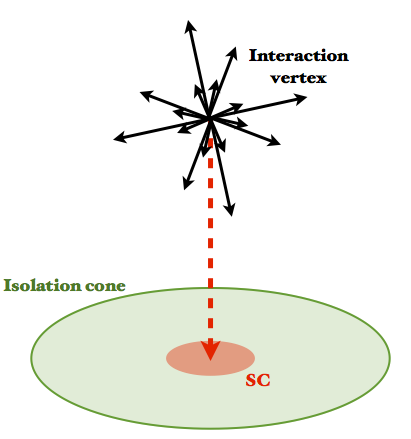
\includegraphics[width=0.45\textwidth]{Figures/RandomCone1.png}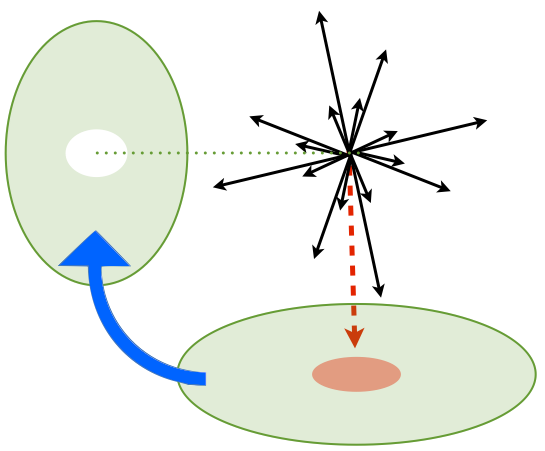
\includegraphics[width=0.55\textwidth]{Figures/RandomCone2.png}
\end{center}
\caption{Illustration of the random cone technique. Under the assumption that the footprint of the photon (red) is completely removed from the isolation sum, the energy deposited in the random-cone area (green in right image) predicts the energy deposited in the isolation cone (green area in left image). \cite{MarcoThesis}}
\label{fig-RandomConeIsolation}
\end{figure}

Figure \ref{fig-signalComparison} shows the comparison of templates from the random cone isolation method and the isolation in MC events which encompass genuine prompt photons and misidentified electrons for each decay channel. We observe a good agreement between data-driven and expected MC templates.   

\begin{figure}
\includegraphics[width=0.5\textwidth]{Plots/signalComparison/MuMu/sigComparison.pdf}
\includegraphics[width=0.5\textwidth]{Plots/signalComparison/EE/sigComparison.pdf}
\begin{center}
\includegraphics[width=0.5\textwidth]{Plots/signalComparison/EMu/sigComparison.pdf}
\end{center}
\caption{Comparison of the shape from random cone isolation and isolated photons identified from generator particle matching in the $\mu^{+}\mu^{-}$, $e^{+}e^{-}$, and $e\mu$ channels.}
\label{fig-signalComparison}
\end{figure}

\subsection{Background estimation using the $\sigma_{i \eta i \eta}$ side-band method} \label{subsec-BackgroundEstimation}

Background events in our template fit are identified as non-prompt photons. We define a template to model our background by selecting photon candidates that fail one selection requirement, which we call the ``side-band" region. The logic behind this method is such that by inverting a particular cut on the photon selection, then we have a sample that is rich in ``photon-like" jets (whereby the hadronisation process resolves to a neutral boosted meson with very little activity around it). In order to model the background correctly, we must select the requirements on the side-band region such that they do not differ too greatly from the full selection, and thus we do not incorrectly reject a genuine jet. 

For the $t\bar{t}+\gamma$ analysis, we create a side-band region by inverting the photon shower-shape ($\sigma_{i\eta i\eta}$) selection cut, thus giving a cut of $0.12 < \sigma_{i \eta i \eta} < 0.20$ where all other photon ID selection requirements still remain the same. When considering a side-band variable, we choose a variable with little to no correlation with our template variable in order to optimise the performance of the method. The shape of the side-band template will then closely resemble the isolation distribution for photons that are not prompt but pass the photon ID requirements. 

We calculate the shower shape of the photon by measuring energy deposits from within a $5 \times 5$ matrix of crystals, centred around the crystal with the largest energy in the super-cluster. As the super-cluster footprint-removal technique removes the super-cluster from the isolation sum, then we have no shared input between the two variables (shower shape and isolation) effectively removing any correlation between the two. However, no two variables are ever truly uncorrelated, and any residual correlation can be attributed to the properties of hadronisation of jets. As our main source of fake photons arises in the form of jets misidentified as photons, we use the supercluster footprint-removed charged hadron isolation (as described in Section \ref{subsec-SCFR}) as our background template variable to discriminate against fake photons.

In Figure \ref{fig-backgroundComparison} we show a comparison of the photon shower shape side-band distributions from our data-driven and MC templates. We observe a good agreement between the distributions.  


\begin{figure}
\includegraphics[width=0.5\textwidth]{Plots/signalComparison/MuMu/bkgdComparison.pdf}
\includegraphics[width=0.5\textwidth]{Plots/signalComparison/EE/bkgdComparison.pdf}
\begin{center}
\includegraphics[width=0.5\textwidth]{Plots/signalComparison/EMu/bkgdComparison.pdf}
\end{center}
\caption{Comparison of the isolation profiles from the side band region and isolation of hadronic photons identified from generator particle matching in the $\mu^{+}\mu^{-}$, $e^{+}e^{-}$, and $e\mu$ channels.}
\label{fig-backgroundComparison}
\end{figure}

\subsection{Fit to charged hadron isolation}

We perform the fit in the SCFR charged hadron isolation less than 20 GeV in order to ensure a good description of background. Loose photon candidates are used for the fit to increase statistics as the dilepton channels are statistically limited. After the fit is computed, the result is corrected by applying the nominal isolation cut on the templates, then computing the true number of genuine photons, misidentified electrons, and jets identified as photons. 

We wish to cross-check our fitting method and we do so by applying it to the collection of simulated samples weighted by their theoretical cross-section and integrated luminosity of the data used in the analysis, whereby creating a pseudo-set of data. By performing the fit on a pseudo-set of data we can cross-reference the results of the fit, photon purity calculation, and cross-reference if the photon purity measurement is in agreement with generator information. We can see the fit templates and fit in Figures \ref{fig-pseudofitTemplates} and \ref{fig-pseudofit}, respectively.


\begin{figure}
\includegraphics[width=0.5\textwidth]{Plots/Fits/TTbarPhotonAnalysis/MuMu/central/pseudoFitTemplate.pdf}
\includegraphics[width=0.5\textwidth]{Plots/Fits/TTbarPhotonAnalysis/EE/central/pseudoFitTemplate.pdf}\\
\begin{center}
\includegraphics[width=0.5\textwidth]{Plots/Fits/TTbarPhotonAnalysis/EMu/central/pseudoFitTemplate.pdf}
\end{center}
\caption{Fit to charged hadron isolation templates with pseudo-data in the $\mu^{+}\mu^{-}$, $e^{+}e^{-}$, and $e\mu$ channels.}
\label{fig-pseudofitTemplates}
\end{figure}

\begin{figure}
\includegraphics[width=0.5\textwidth]{Plots/Fits/TTbarPhotonAnalysis/MuMu/central/pseudoFit.pdf}
\includegraphics[width=0.5\textwidth]{Plots/Fits/TTbarPhotonAnalysis/EE/central/pseudoFit.pdf}\\
\begin{center}
\includegraphics[width=0.5\textwidth]{Plots/Fits/TTbarPhotonAnalysis/EMu/central/pseudoFit.pdf}
\end{center}
\caption{Fit to charged hadron isolation with pseudo-data in the $\mu^{+}\mu^{-}$, $e^{+}e^{-}$, and $e\mu$ channels.}
\label{fig-pseudofit}
\end{figure}

In an attempt to verify that the fit works well across a range of potential photon purity values, and thus not having a bias towards predicted values, we perform the fit while varying the photon purity value. Due to the $t\bar{t}+\gamma$ simulated sample comprising predominantly prompt photon events, by scaling the $t\bar{t}+\gamma$ contribution we vary the photon purity value. Figure \ref{fig-photonPurityComparison} shows a comparison of the photon purity value and and the corresponding value measured by the fit to the charged hadron isolation. 


\begin{figure}
\includegraphics[width=0.3\textwidth]{Plots/purityComparison/MuMu/photonPurity.pdf}
\includegraphics[width=0.3\textwidth]{Plots/purityComparison/EE/photonPurity.pdf}
\includegraphics[width=0.3\textwidth]{Plots/purityComparison/EMu/photonPurity.pdf}
\caption{Comparison of the photon purity of pseudo-data sets to the values measured by the fit to the charged hadron isolation in the $\mu^{+}\mu^{-}$, $e^{+}e^{-}$, and $e\mu$ channels.}
\label{fig-photonPuritiyComparison}
\end{figure}

We can see the template fit to the charged hadron isolation for the full data set in Figure \ref{fig-fitTemplates} for each decay channel. After the fit is conducted, we find photon purity values of $0.634 \pm 0.054$, $0.634 \pm 0.054$, and $0.634 \pm 0.054$ (including statistical uncertainties only for pseudo-data) compared to photon purity values of $0.634 \pm 0.054$, $0.634 \pm 0.054$, and $0.634 \pm 0.054$ from generator level information, in the $\mu^{+}\mu^{-}$, $e^{+}e^{-}$, and $e\mu$ channels, respectively. 

% Statistical uncertainty given by RooFit does not include variation of the templates but only
% uncertainty of data. However since templates are data-driven and suffer from low statistics
% we have to take this uncertainty into account. We perform pseudo experiments where for
% data, isolated and hadronic photon templates in each bin the value is randomly chosen by
% Poisson distribution with mean of the bin content in the original histogram. The width of
% the distribution of the photon purity in these pseudo experiments is taken as the statistical
% uncertainty. The photon purity is calculated using only the portion of the isolation distribution
% that passes the original 5 GeV isolation cut. From the fit, the photon purity is measured to be
% 0.57 ± 0.06 in the e + jets channel and 0.53 ± 0.06 in the μ + jets channel.

\begin{figure}
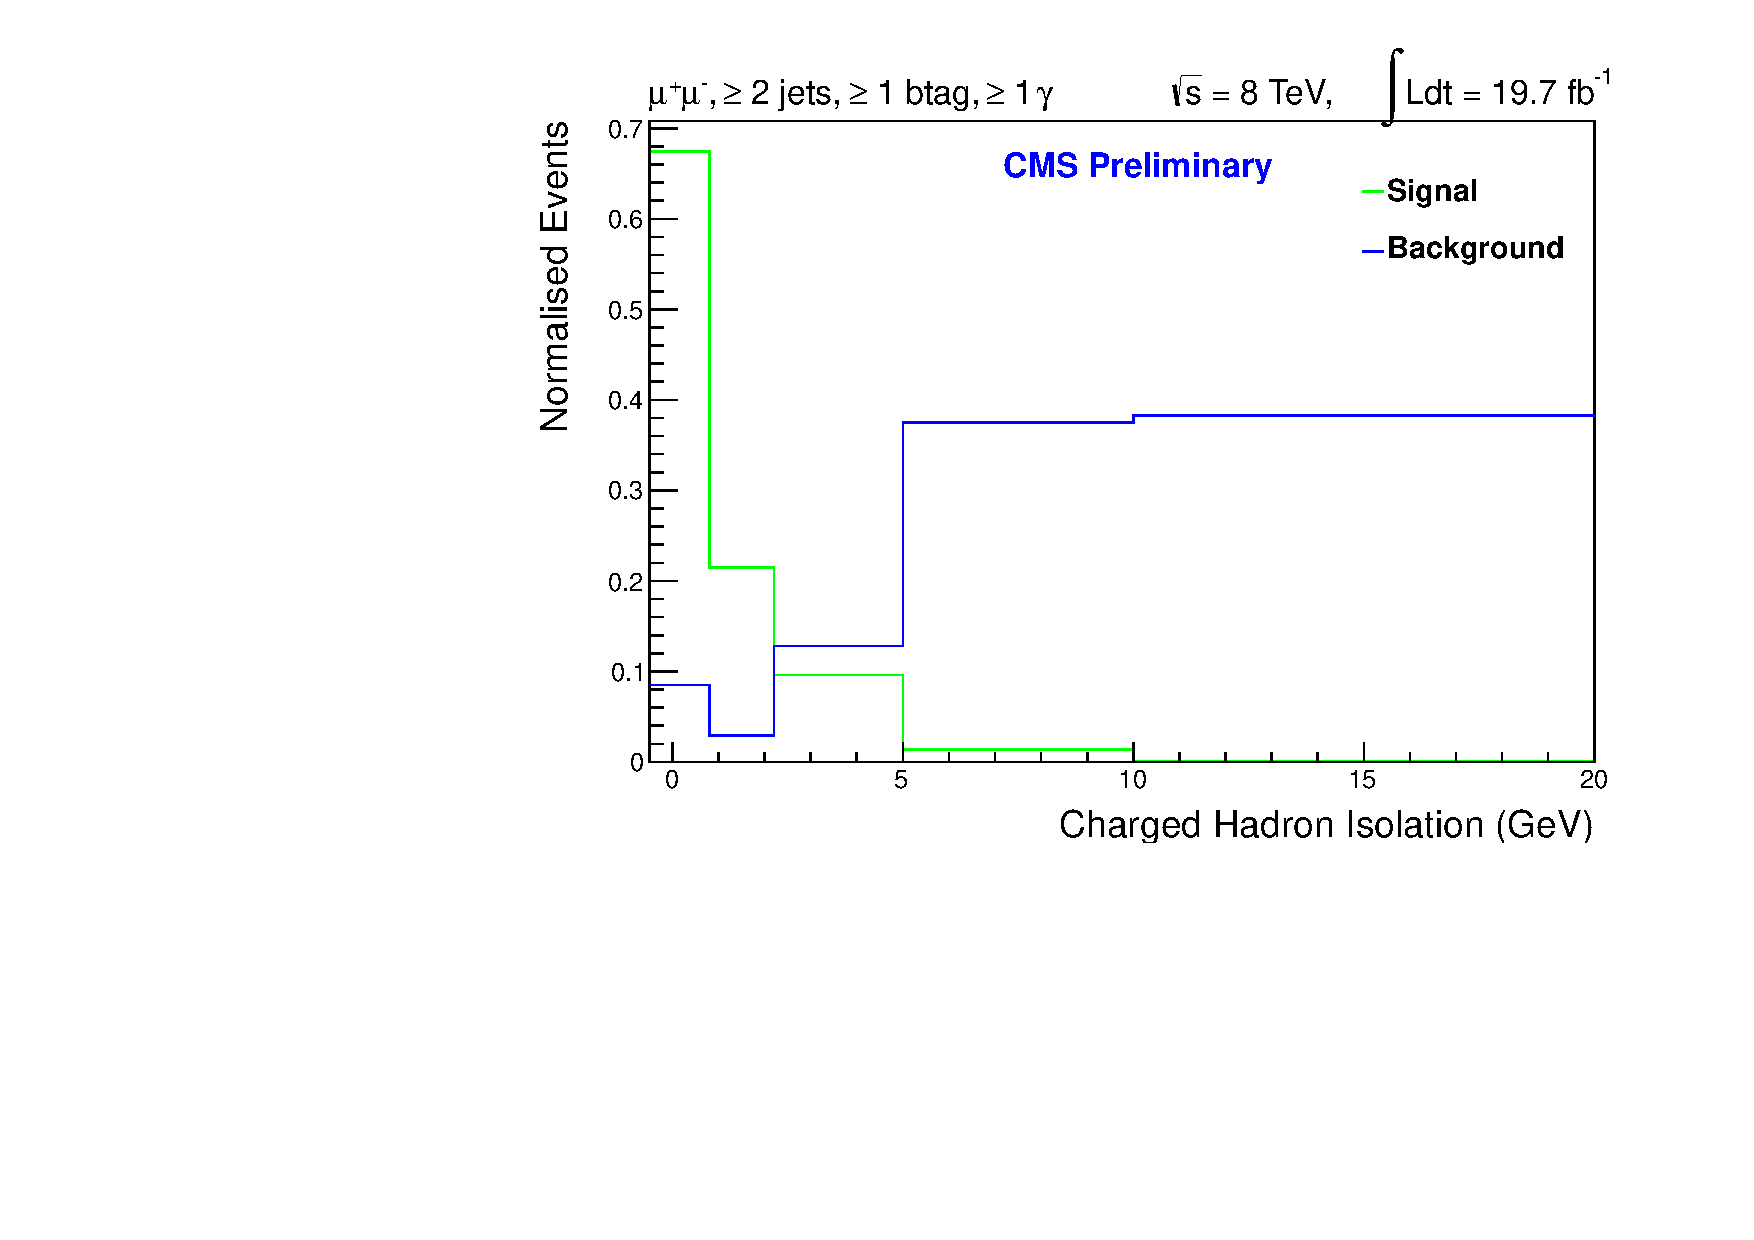
\includegraphics[width=0.5\textwidth]{Plots/Fits/TTbarPhotonAnalysis/MuMu/central/FitTemplate.pdf}
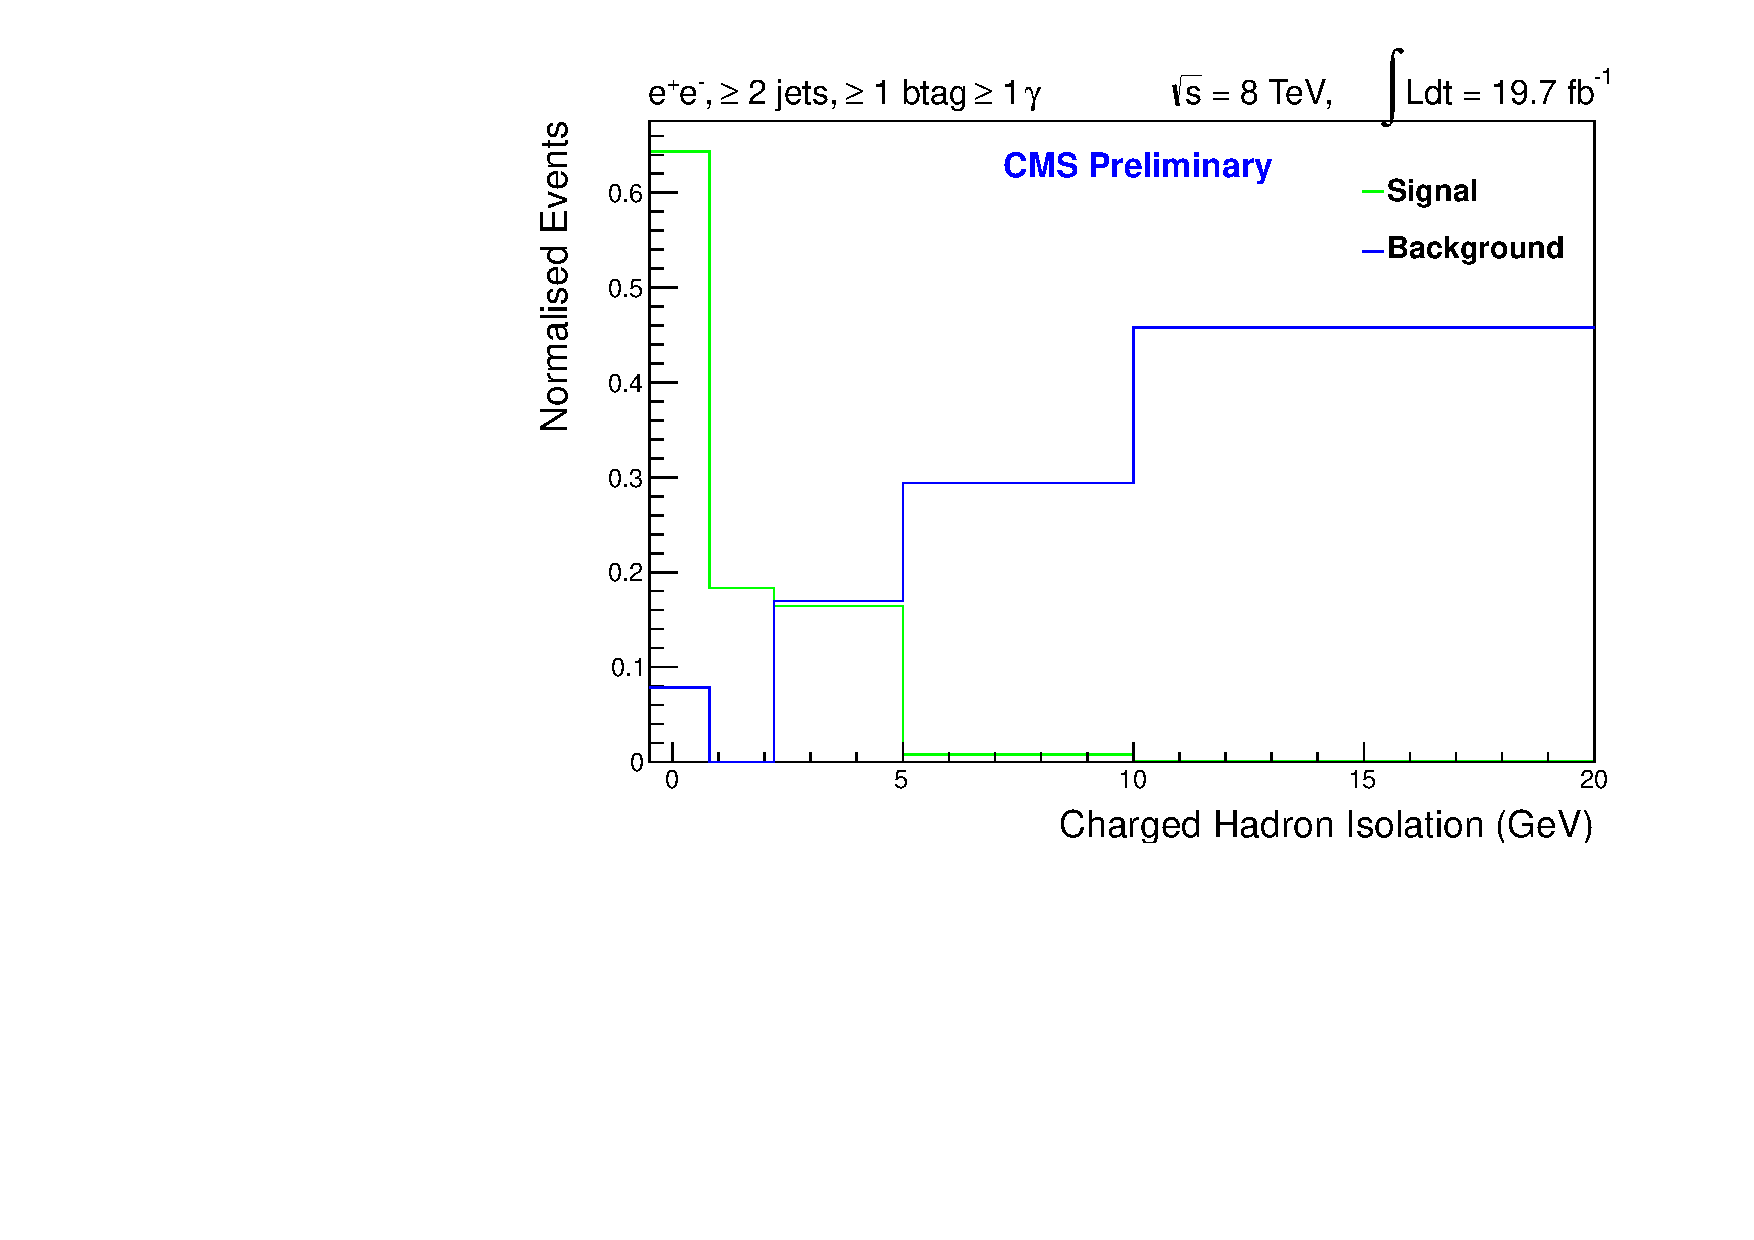
\includegraphics[width=0.5\textwidth]{Plots/Fits/TTbarPhotonAnalysis/EE/central/FitTemplate.pdf}\\
\begin{center}
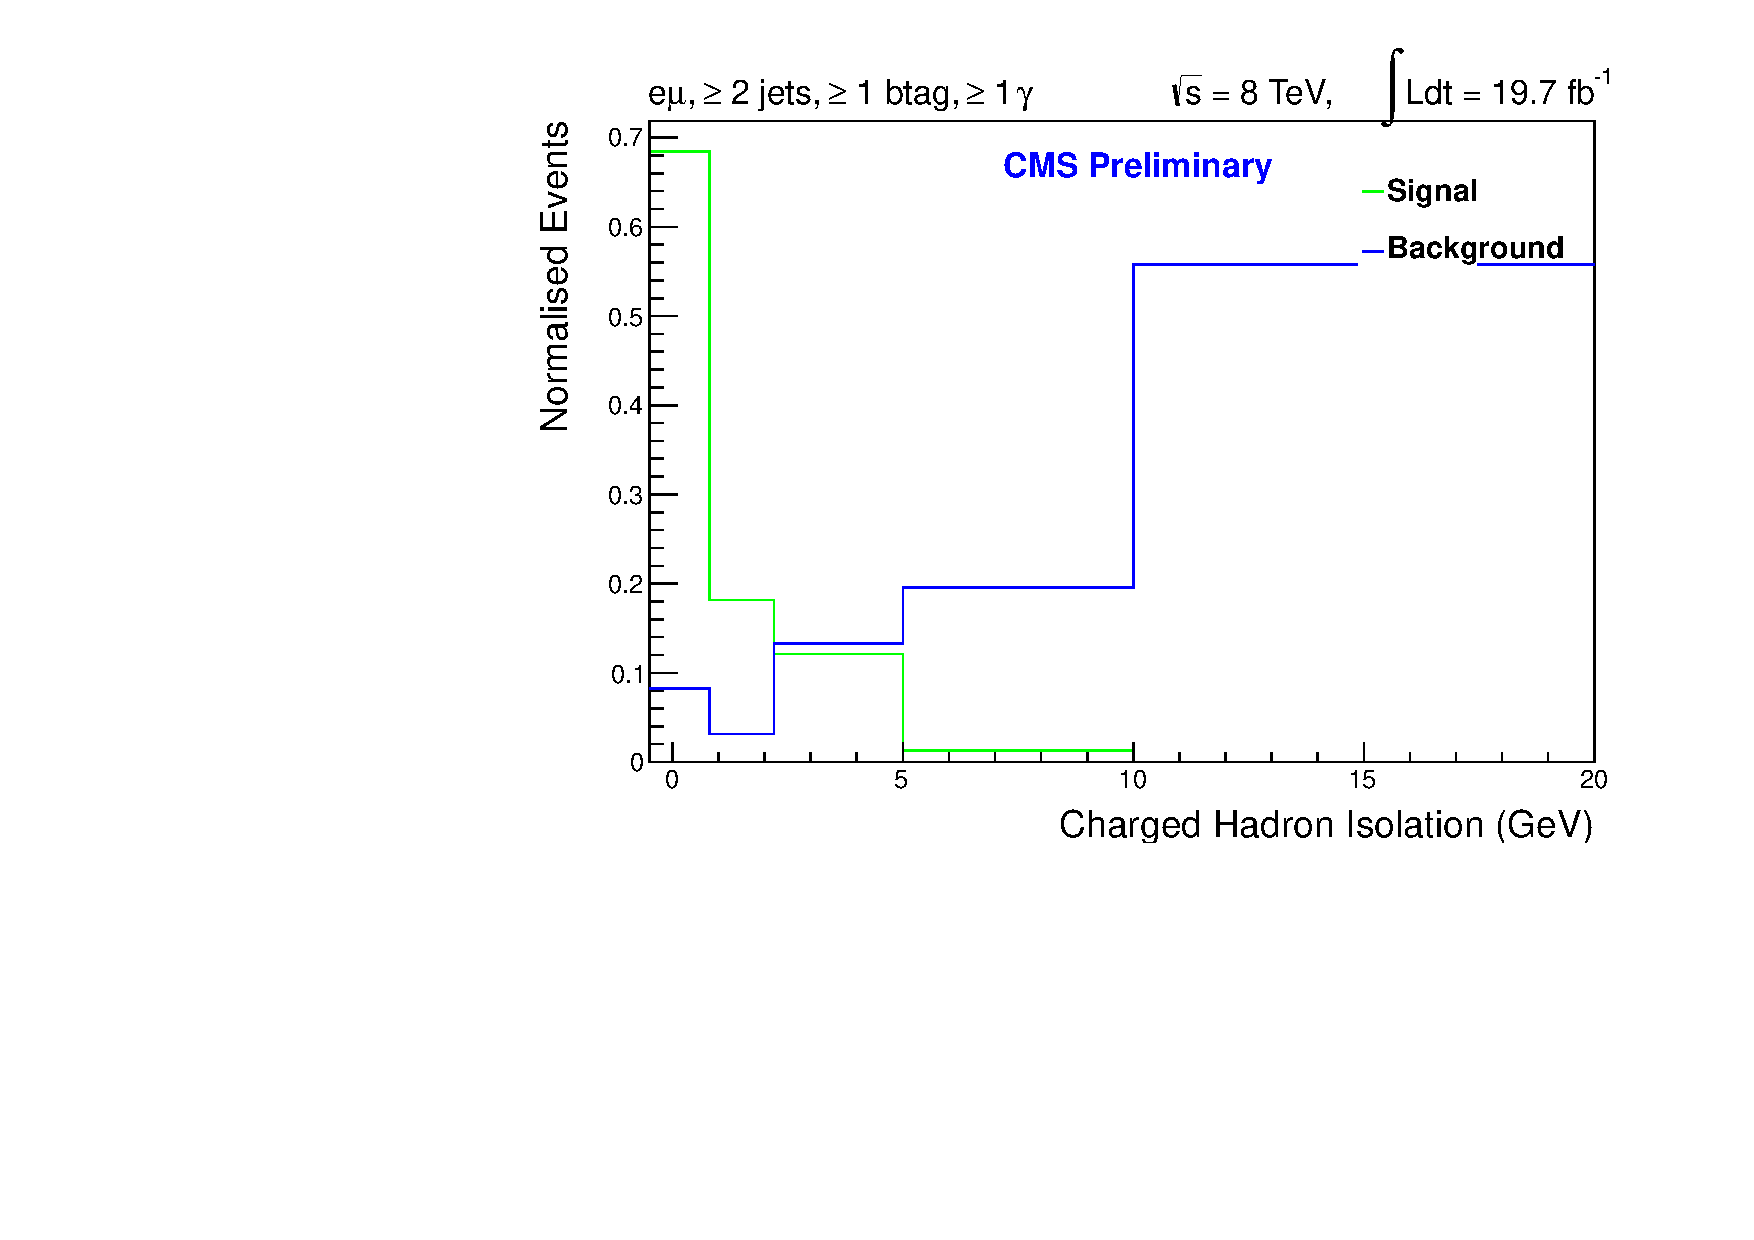
\includegraphics[width=0.5\textwidth]{Plots/Fits/TTbarPhotonAnalysis/EMu/central/FitTemplate.pdf}
\end{center}
\caption{Fit to charged hadron isolation templates in the $\mu^{+}\mu^{-}$, $e^{+}e^{-}$, and $e\mu$ channels.}
\label{fig-fitTemplates}
\end{figure}

\begin{figure}
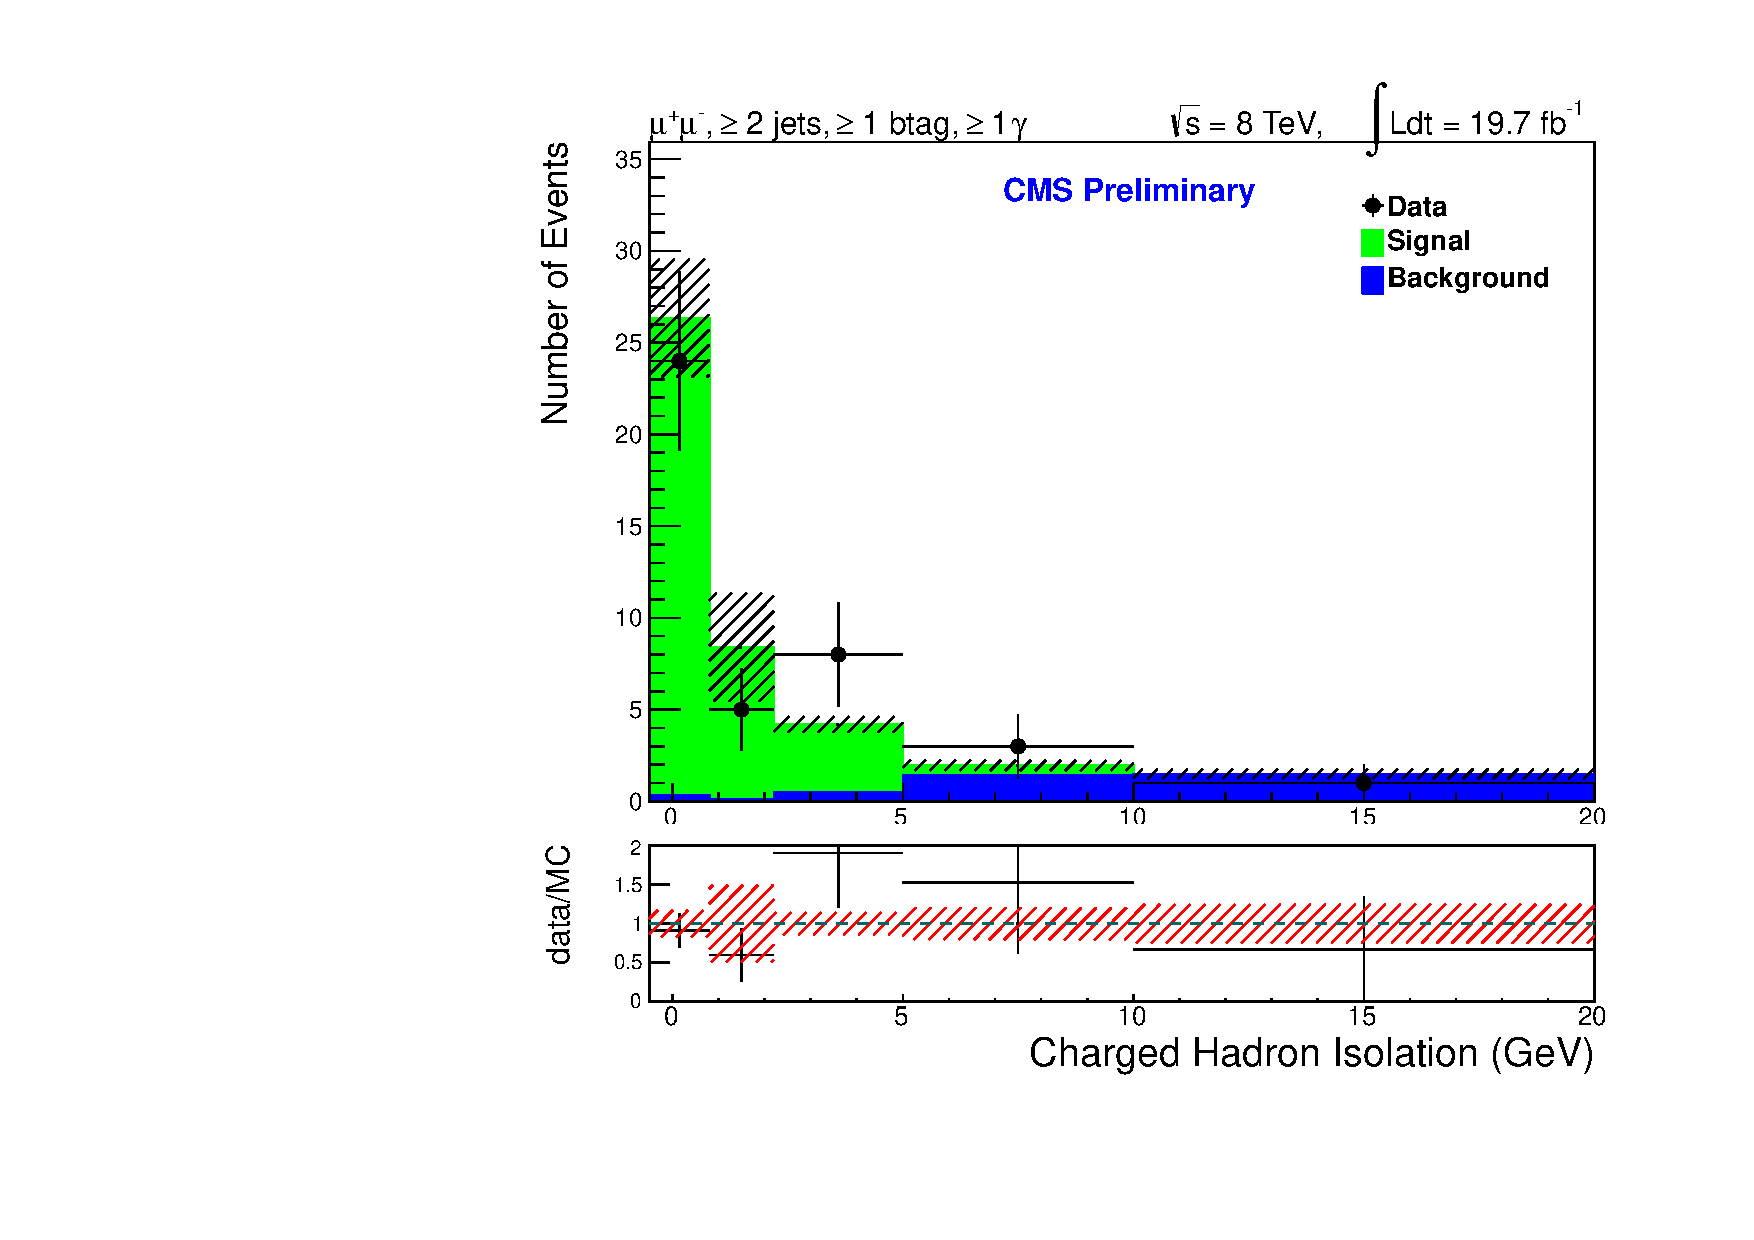
\includegraphics[width=0.5\textwidth]{Plots/Fits/TTbarPhotonAnalysis/MuMu/central/Fit.pdf}
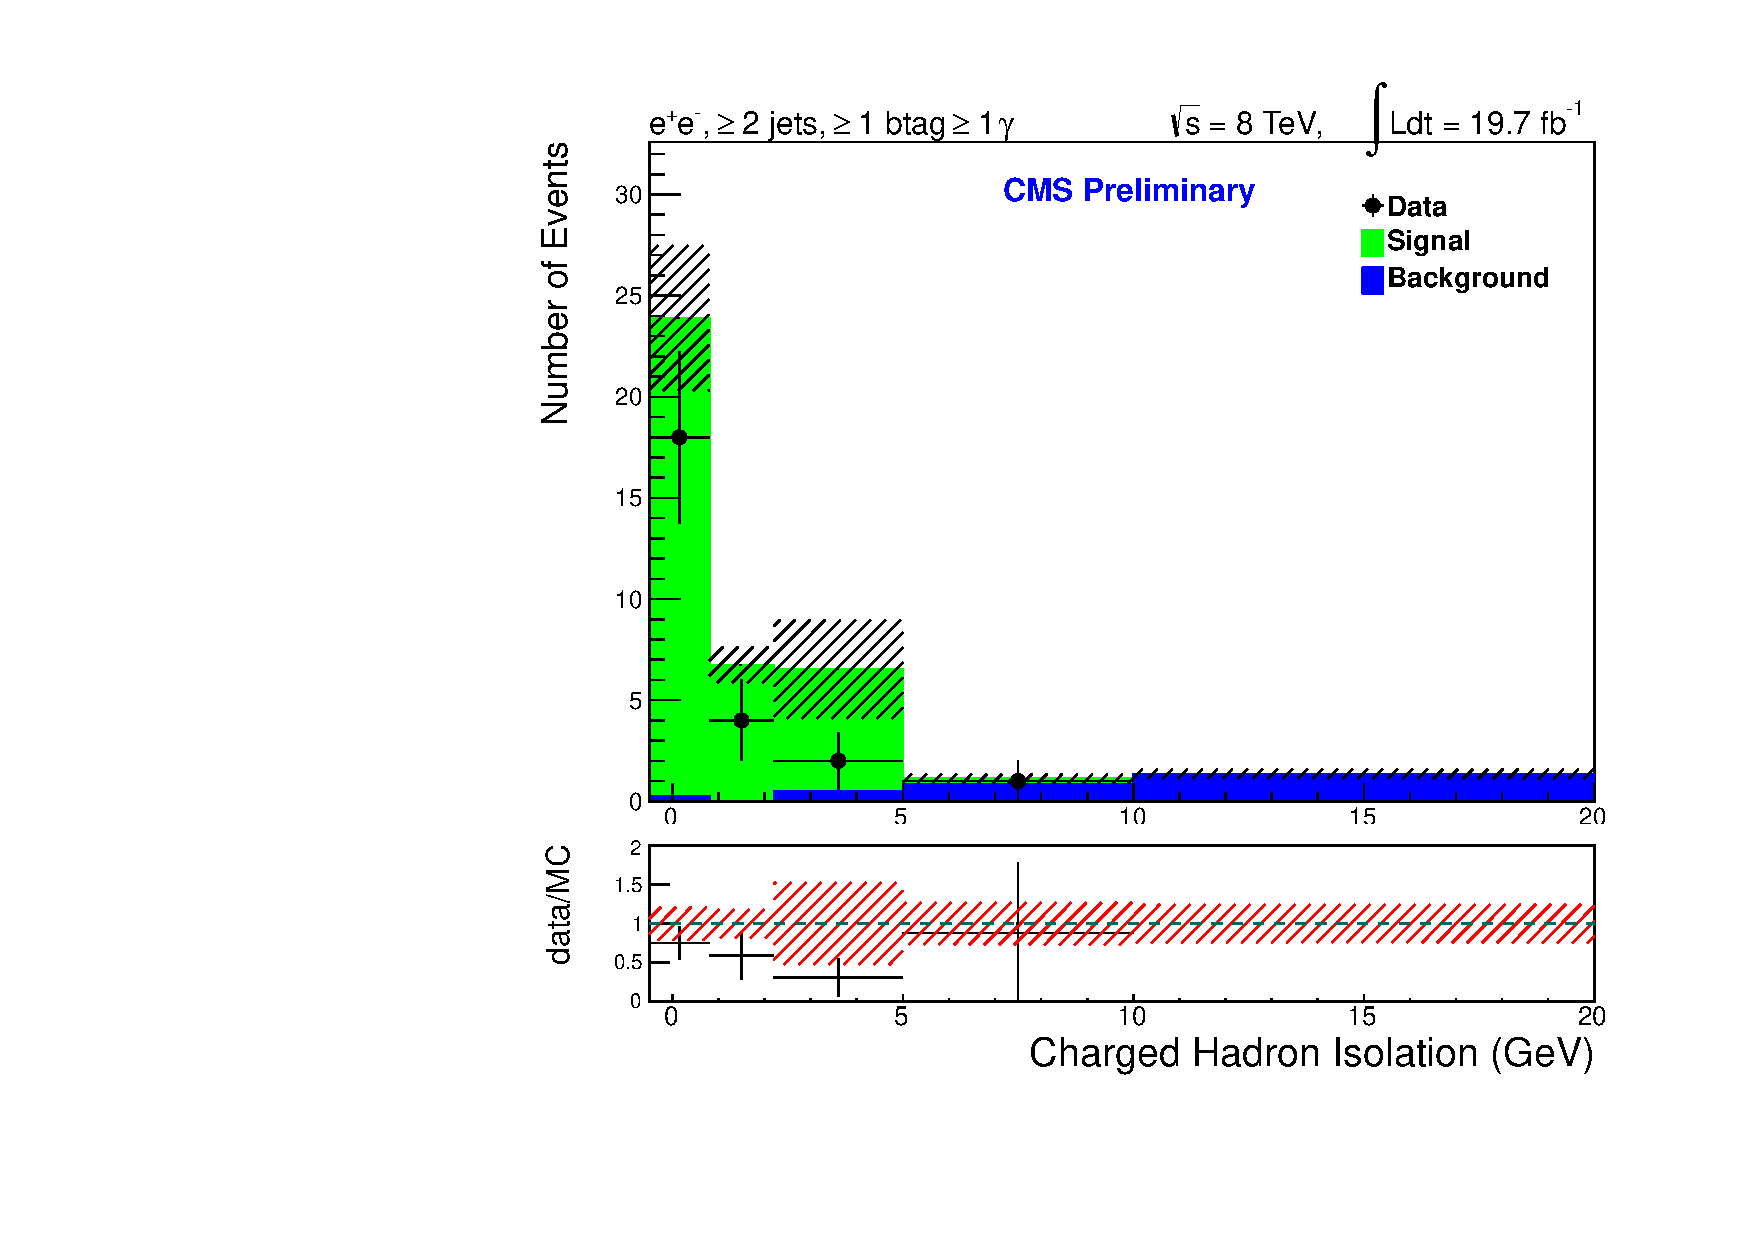
\includegraphics[width=0.5\textwidth]{Plots/Fits/TTbarPhotonAnalysis/EE/central/Fit.pdf}\\
\begin{center}
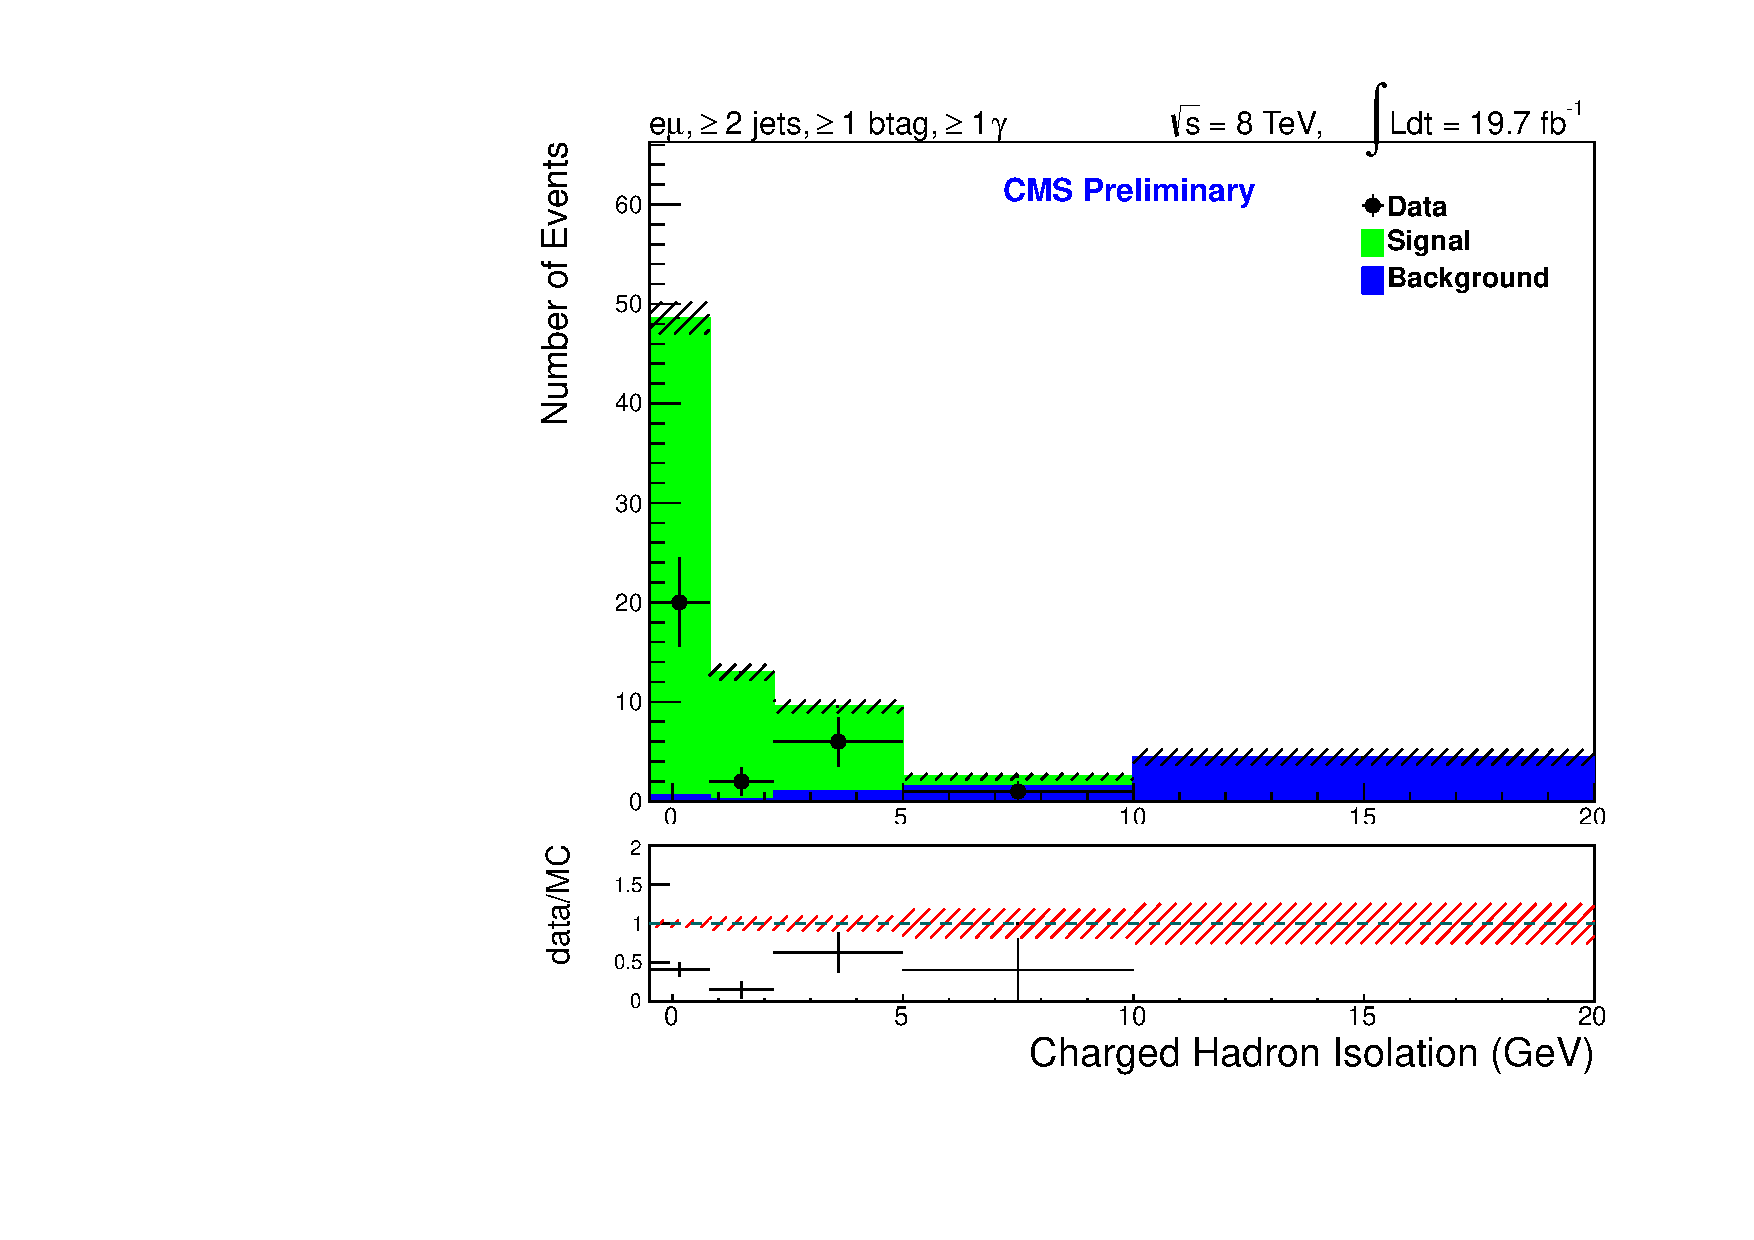
\includegraphics[width=0.5\textwidth]{Plots/Fits/TTbarPhotonAnalysis/EMu/central/Fit.pdf}
\end{center}
\caption{Fit to charged hadron isolation in the $\mu^{+}\mu^{-}$, $e^{+}e^{-}$, and $e\mu$ channels.}
\label{fig-fits}
\end{figure}



\begin{sidewaystable} 
\begin{center}
\begin{tabular}{|l|c|}
\hline
	\textbf{Dataset} & \textbf{Integrated Luminosity ($pb^{-1}$)}\\
\hline
	/DoubleMuParked/Run2012A-22Jan2013-v1/AOD  & 876 \\
	/DoubleMuParked/Run2012B-22Jan2013-v1/AOD  & 4412 \\
	/DoubleMuParked/Run2012C-22Jan2013-v1/AOD  & 7017 \\
	/DoubleMuParked/Run2012D-22Jan2013-v1/AOD  & 7369 \\
\hline
	Total & 19.7\\	
\hline
	/DoubleElectron/Run2012A-22Jan2013-v1/AOD  & 875 \\
	/DoubleElectron/Run2012B-22Jan2013-v1/AOD  & 4412 \\
	/DoubleElectron/Run2012C-22Jan2013-v1/AOD  & 7055 \\
	/DoubleElectron/Run2012D-22Jan2013-v1/AOD  & 7369 \\
\hline
	Total & 19.7\\	
\hline
	/MuEG/Run2012A-22Jan2013-v1/AOD  & 876 \\
	/MuEG/Run2012B-22Jan2013-v1/AOD  & 4411 \\
	/MuEG/Run2012C-22Jan2013-v1/AOD  & 7055 \\
	/MuEG/Run2012D-22Jan2013-v1/AOD  & 7360 \\
\hline
	Total & 19.7\\	
\hline	
\end{tabular}	
\end{center}
\caption{Dataset information for each run in each respective decay channel.}
\label{tab-datasets}
\end{sidewaystable}

\section{Number of signal events in data} \label{sec-SigEventsInData}

Tables \ref{tab-SigPhotonsMuMu}, \ref{tab-SigPhotonsEE}, and \ref{tab-SigPhotonsEMu} show the number of photons after full selection broken down into categories of origin for individual MC samples, shown for each $t\bar{t}+\gamma$ decay channel. This method is used in order to extract the true number of signal $t\bar{t}+\gamma$ events to be used as a variable in the cross-section calculation. 

We divide the resultant photons into three categories: genuine prompt and isolated photons, isolated misidentified electrons, and jets reconstructed as photons. Individual simulated samples contribute to each category differently, therefore we introduce scale factors to correct for mismodelling of the three categories. 

\begin{table}
\begin{center}
\resizebox{\columnwidth}{!} {
\begin{tabular}{l|ccc|c}
\hline
	\textbf{Sample} & \textbf{Genuine Photon} & \textbf{MisID Electron} & \textbf{Hadronic} & \textbf{Total} \\
\hline
$t\bar{t}+\gamma$  & 11.5597 $\pm$ 0.677995 & 0 $\pm$ 0 & 6.41284 $\pm$ 0.508448 & 17.9725 $\pm$ 0.847465 \\
$t\bar{t}+jets$  & 1.84297 $\pm$ 0.299532 & 0 $\pm$ 0 & 4.03535 $\pm$ 0.454349 & 5.87832 $\pm$ 0.544199 \\
$W+\gamma$  & 0 $\pm$ 0 & 0 $\pm$ 0 & 0 $\pm$ 0 & 0 $\pm$ 0 \\
$W+jets$  & 0 $\pm$ 0 & 0 $\pm$ 0 & 0 $\pm$ 0 & 0 $\pm$ 0 \\
$Z+\gamma$  & 4.97919 $\pm$ 1.8975 & 0 $\pm$ 0 & 0.644821 $\pm$ 0.644821 & 5.62401 $\pm$ 2.00407 \\
$Z+jets$  & 3.97058 $\pm$ 3.06254 & 0 $\pm$ 0 & 0 $\pm$ 0 & 3.97058 $\pm$ 3.06254 \\
Single Top  & 0 $\pm$ 0 & 0 $\pm$ 0 & 0 $\pm$ 0 & 0 $\pm$ 0 \\
Diboson  & 0.296448 $\pm$ 0.112047 & 0 $\pm$ 0 & 0 $\pm$ 0 & 0.296448 $\pm$ 0.112047 \\
\hline
Total  & 22.9453 $\pm$ 3.6816 & 0 $\pm$ 0 & 11.093 $\pm$ 0.938482 & 34.0383 $\pm$ 3.79933 \\
Data  & --- & --- & --- & 36 $\pm$ 6 \\
\hline	
\end{tabular}
}
\end{center}
\caption{Simulated samples categorised by origin of reconstructed origin after nominal selection in the $\mu^+\mu^-$ channel. Events are normalized by process theoretical cross-sections. Data-driven QCD sample is not expected to have signal photons or electrons. All errors are statistical.}
\label{tab-SigPhotonsMuMu}
\end{table}	

\begin{table}
\begin{center}
\resizebox{\columnwidth}{!} {
\begin{tabular}{l|ccc|c}
\hline
	\textbf{Sample} & \textbf{Genuine Photon} & \textbf{MisID Electron} & \textbf{Hadronic} & \textbf{Total} \\
\hline
$t\bar{t}+\gamma$  & 11.5597 $\pm$ 0.677995 & 0 $\pm$ 0 & 6.41284 $\pm$ 0.508448 & 17.9725 $\pm$ 0.847465 \\
$t\bar{t}+jets$  & 1.84297 $\pm$ 0.299532 & 0 $\pm$ 0 & 4.03535 $\pm$ 0.454349 & 5.87832 $\pm$ 0.544199 \\
$W+\gamma$  & 0 $\pm$ 0 & 0 $\pm$ 0 & 0 $\pm$ 0 & 0 $\pm$ 0 \\
$W+jets$  & 0 $\pm$ 0 & 0 $\pm$ 0 & 0 $\pm$ 0 & 0 $\pm$ 0 \\
$Z+\gamma$  & 4.97919 $\pm$ 1.8975 & 0 $\pm$ 0 & 0.644821 $\pm$ 0.644821 & 5.62401 $\pm$ 2.00407 \\
$Z+jets$  & 3.97058 $\pm$ 3.06254 & 0 $\pm$ 0 & 0 $\pm$ 0 & 3.97058 $\pm$ 3.06254 \\
Single Top  & 0 $\pm$ 0 & 0 $\pm$ 0 & 0 $\pm$ 0 & 0 $\pm$ 0 \\
Diboson  & 0.296448 $\pm$ 0.112047 & 0 $\pm$ 0 & 0 $\pm$ 0 & 0.296448 $\pm$ 0.112047 \\
\hline
Total  & 18.2628 $\pm$ 1.90184 & 0.0578557 $\pm$ 0.0578557 & 13.4295 $\pm$ 2.97618 & 31.7501 $\pm$ 3.53242 \\
Data  & --- & --- & --- & 26 $\pm$ 5.09902 \\
\hline	
\end{tabular}
}
\end{center}
\caption{Simulated samples categorised by origin of reconstructed origin after nominal selection in the $e^+e^-$ channel. Events are normalized by process theoretical cross-sections. Data-driven QCD sample is not expected to have signal photons or electrons. All errors are statistical.}
\label{tab-SigPhotonsEE}
\end{table}	

\begin{table}
\begin{center}
\resizebox{\columnwidth}{!} {
\begin{tabular}{l|ccc|c}
\hline
	\textbf{Sample} & \textbf{Genuine Photon} & \textbf{MisID Electron} & \textbf{Hadronic} & \textbf{Total} \\
\hline
$t\bar{t}+\gamma$  & 29.3472 $\pm$ 1.09904 & 0 $\pm$ 0 & 13.3482 $\pm$ 0.73033 & 42.6954 $\pm$ 1.31957 \\
$t\bar{t}+jets$  & 3.23091 $\pm$ 0.403224 & 0.0641023 $\pm$ 0.0641023 & 8.4431 $\pm$ 0.633878 & 11.7381 $\pm$ 0.75399 \\
$W+\gamma$  & 0 $\pm$ 0 & 0 $\pm$ 0 & 0 $\pm$ 0 & 0 $\pm$ 0 \\
$W+jets$  & 0 $\pm$ 0 & 0 $\pm$ 0 & 0 $\pm$ 0 & 0 $\pm$ 0 \\
$Z+\gamma$  & 0 $\pm$ 0 & 0 $\pm$ 0 & 0 $\pm$ 0 & 0 $\pm$ 0 \\
$Z+jets$  & 0 $\pm$ 0 & 0 $\pm$ 0 & 0 $\pm$ 0 & 0 $\pm$ 0 \\
Single Top  & 0.270833 $\pm$ 0.270833 & 0 $\pm$ 0 & 0.70516 $\pm$ 0.70516 & 0.975993 $\pm$ 0.755381 \\
Diboson  & 0.176487 $\pm$ 0.176487 & 0 $\pm$ 0 & 0 $\pm$ 0 & 0.176487 $\pm$ 0.176487 \\
\hline
Total  & 33.2019 $\pm$ 1.22724 & 0.0641023 $\pm$ 0.0641023 & 22.4965 $\pm$ 1.19684 & 55.7625 $\pm$ 1.71542 \\
Data  & --- & --- & --- & 28 $\pm$ 5.2915 \\
\hline	
\end{tabular}
}
\end{center}
\caption{Simulated samples categorised by origin of reconstructed origin after nominal selection in the $e\mu$ channel. Events are normalized by process theoretical cross-sections. Data-driven QCD sample is not expected to have signal photons or electrons. All errors are statistical.}
\label{tab-SigPhotonsEMu}
\end{table}	

The behaviour of the TTJets, WJets, ZJets, and DiBoson samples is well understood and has been cross-checked, and corrected, by different template fits to data. Thus leaving the contribution from the TTGamma and VGamma (the combination of WGamma and ZGamma) samples that are not as well understood, both being the largest contributors to our signal process. The VGamma sample is normalised to its NLO theoretical cross-section, and known to potentially be mismodelled to the order of 20\% \cite{PhysRevD.89.092005}. The VGamma sample has the second largest contribution to signal events out of all MC samples, and therefore it is critical that we cross-check the normalisation before including it. Single top events are also well modelled, however they do not contribute significantly to the signal process.

We are thus left we three unknowns:

\begin{itemize}
	\item TTGamma scale factor (or normalisation, the main unknown) 
	\item VGamma scale factor
	\item Jet to photon misidentification scale factor
\end{itemize}

From the events derived from data we can define the photon purity, $\pi_{e\gamma}$, taken from the charged hadron isolation data-driven template fit, which also includes electrons misidentified as photons. We can also compute the $t\bar{t}$ purity, $\pi_{t\bar{t}}$, and the total number of selected events in data. For every measured quantity we attach an associated uncertainty and propagate through to the unknown quantities described above. By relating the known quantities to the unknowns we can construct a likelihood function $\lumi(SF_{t\bar{t}+\gamma},SF_{V+\gamma},SF_{jet\to\gamma}) = e^{-\chi^2/2}$, where $\chi^2$ is the sum of the three chi-squared terms for each scale factor, given as   

\begin{equation}
\chi^2(SF_{t\bar{t}+\gamma},SF_{V+\gamma},SF_{jet\to\gamma}) = \frac{\left(\pi^{data}_{e\gamma} - \pi^{MC}_{e\gamma}\right)^2}{\sigma^2_{\pi_{e\gamma}}} + \frac{\left(\pi^{data}_{t\bar{t}} - \pi^{MC}_{t\bar{t}}\right)^2}{\sigma^2_{\pi_{t\bar{t}}}} + \frac{\left(N^{data}_{events} - N^{MC}_{events}\right)^2}{\sigma^2_{N_{events}}}
\end{equation}

We use the three unknown quantities in order to correct event counts from relevant contributions in simulation. These quantities are: $\pi_{e\gamma}^{MC}$, ratio of events with a reconstructed photon matched to an isolated electron or photon and all events in simulation, $\pi_{t\bar{t}}^{MC}$ the ratio of top pair events and all events from simulation, and $\pi_{events}^{MC}$ the total number of selected events in MC. The values of these parameters for both data and MC can be seen in Table \ref{tab-likelihoodVariables}	

As we wish to find the combination of parameters with the best likelihood, we perform a scan over possible values of the parameters. We then compute the negative log-likelihood ratio by maximising the likelihood where we fix one parameter to a specific value, and then taking the ratio of the maximum likelihood value at this point to the global maximum likelihood. We take the 68\% confidence interval to be the range of values for which the negative log-likelihood ratio is less than 0.5. Figures \ref{fig-SFLikelihoodFitsMuMu}, \ref{fig-SFLikelihoodFitsMuMu}, and \ref{fig-SFLikelihoodFitsMuMu} show the negative log-likelihood ratio distributions for the $\mu^+\mu^-$, $e^+e^-$, and $e\mu$ channels, respectively. 

\begin{table}
\begin{center}
\begin{tabular}{l|cc|cc|cc}
\hline
	& \multicolumn{2}{c|}{$\mu^{+}\mu^{-}$} & \multicolumn{2}{c|}{$e^{+}e^{-}$} & \multicolumn{2}{c}{$e\mu$} \\
	& data & MC & data & MC & data & MC \\
\hline
	Photon purity & & & & & &\\
	Top purity & & & & & &\\
	$N_{events}$ data & & & & & & \\
\hline	
\end{tabular}
\end{center}
\caption{Measured quantities used in the likelihood fit for the $\mu^{+}\mu^{-}$, $e^{+}e^{-}$, and $e\mu$ channels.}
\label{tab-likelihoodVariables}
\end{table}		

\begin{figure}
\includegraphics[width=0.3\textwidth]{Plots/likelihoodfits/MuMu/ttgamma_likelihood_fit.pdf}
\includegraphics[width=0.3\textwidth]{Plots/likelihoodfits/MuMu/vgamma_likelihood_fit.pdf}
\includegraphics[width=0.3\textwidth]{Plots/likelihoodfits/MuMu/jgamma_likelihood_fit.pdf}
\caption{Likelihood distributions for the $t\bar{t}+\gamma$, $V+\gamma$, and $jets\to \gamma$ scale factors in the $\mu^{+}\mu^{-}$ channel.}
\label{fig-SFLikelihoodFitsMuMu}
\end{figure}

\begin{figure}
\includegraphics[width=0.3\textwidth]{Plots/likelihoodfits/EE/ttgamma_likelihood_fit.pdf}
\includegraphics[width=0.3\textwidth]{Plots/likelihoodfits/EE/vgamma_likelihood_fit.pdf}
\includegraphics[width=0.3\textwidth]{Plots/likelihoodfits/EE/jgamma_likelihood_fit.pdf}
\caption{Likelihood distributions for the $t\bar{t}+\gamma$, $V+\gamma$, and $jets\to \gamma$ scale factors in the $e^{+}e^{-}$ channel.}
\label{fig-SFLikelihoodFitsEE}
\end{figure}

\begin{figure}
\includegraphics[width=0.3\textwidth]{Plots/likelihoodfits/EMu/ttgamma_likelihood_fit.pdf}
\includegraphics[width=0.3\textwidth]{Plots/likelihoodfits/EMu/vgamma_likelihood_fit.pdf}
\includegraphics[width=0.3\textwidth]{Plots/likelihoodfits/EMu/jgamma_likelihood_fit.pdf}
\caption{Likelihood distributions for the $t\bar{t}+\gamma$, $V+\gamma$, and $jets\to \gamma$ scale factors in the $e\mu$ channel.}
\label{fig-SFLikelihoodFitsEMu}
\end{figure}



We find that the best agreement is achieved for these values of parameters, with errors from the width of the likelihood, are $SF_{t\bar{t}+\gamma} = 1.16 \pm 0.26$, $SF_{V+\gamma} = 0.95 \pm 0.85$, $SF_{jet\to\gamma} = 1.17 \pm 0.19$ for the $\mu^+\mu^-$ channel, $SF_{t\bar{t}+\gamma} = 0.89 \pm 0.21$, $SF_{V+\gamma} = 1.13 \pm 0.45$, $SF_{jet\to\gamma} = 1.22 \pm  0.18$ for the $e^+e^-$ channel, and $SF_{t\bar{t}+\gamma} = 0.89 \pm 0.21$, $SF_{V+\gamma} = 1.13 \pm 0.45$, $SF_{jet\to\gamma} = 1.22 \pm 0.18$ for the $e\mu$ channel. Therefore, we see an excellent agreement between the photon purity, fraction of top events, and number of events in simulation and in data. Tables \ref{}, \ref{}, \ref{} show the number of events from simulation scaled to the results of the likelihood fit.  


\section{Signal Acceptance Calculation} \label{subsec-SignalAcceptanceCalculation}

%  Additionally,
% the acceptance can be split into two parts, the portion coming from the branching fraction of
% the tt pair, and the portion coming from the kinematic phase space requirements.


The acceptance calculation for this analysis differs from usual inclusive cross section measurements because we measure ratio of cross sections. We measure the both the efficiency and acceptance from simulation, where the acceptance is determined at generator level by requiring events to lie within the phase space chosen for the analysis. We define events to contain exactly two oppositely-signed leptons (excluding $\tau$ leptons) in the visible phase space. For muons, we require a transverse momentum greater than 20 GeV and to lie within a pseudorapidity region of $|\eta| < 2.4$, excluding the region of $1.4442 < \eta < 1.5660$ between the barrel and endcaps. Similarly, the visible phase space for electrons lies in the requirement of a transverse momentum greater than 20 GeV and $|\eta| < 2.4$. We require the MET to be greater than 20 GeV. Finally, we require the selection of generated photon with transverse energy greater than 25 GeV and lie in the pseudorapidity region $|\eta| < 1.4442$ (the barrel region). We define the acceptance to be the fraction of generated events that pass these generator level cuts. 


The event selection is chosen to make use of this fact: two steps (top selection and photon selection) are done sequentially. For the inclusive $t\bar{t}$ process, we start with number of generated events (within some fiducial phase space) and count how many events are left after top event selection. The acceptance times efficiency is defined for the $t\bar{t}$ top selection as:

\begin{equation}
	(\epsilon \cdot A)_{t\bar{t}}^{top} = \frac{N_{t\bar{t}.preselection}}{N_{t\bar{t}.generated}} 
\end{equation}

This gives the acceptance times efficiency of the inclusive $t\bar{t}$ process to be $(\epsilon \cdot A)_{t\bar{t}}^{top} =   \pm  (stat.)$ in the di-muon channel, $(\epsilon \cdot A)_{t\bar{t}}^{top} =  \pm  (stat.)$ in the di-electron channel, and $(\epsilon \cdot A)_{t\bar{t}}^{top} =  \pm  (stat.)$ in the mixed final state.

We note that the branching fraction for the $t\bar{t}+\gamma$ signal is different to normal $t\bar{t}$ production, and is due to the way in which the signal is defined.  We apply tighter generator requirements to jets than leptons, resulting in the relative contribution from the semilaptonic and dileptonic final states being increased within the $t\bar{t}+\gamma$ MC sample, compared to the contribution from the all hadronic final state. We calculate the branching fraction of $t\bar{t}+\gamma$ production if measured from simulation as the total number of events generated with exactly two oppositely-signed leptons (excluding $\tau$ leptons) divided by the total number of generated events. 

\begin{equation}
\mathcal{BR}_{t\bar{t}+\gamma} = \frac{N_{2. lep.}^{t\bar{t}+\gamma}}{N_{Tot. gen.}^{t\bar{t}+\gamma}}
\end{equation} 

We define the kinematic acceptance to be the number of events passing the generator level requirements divided by the number of events generated with exactly two oppositely-signed leptons.

\begin{equation}
A_{t\bar{t}+\gamma}^{kin.} = \frac{N_{t\bar{t}+\gamma}^{gen. fid.}}{N_{t\bar{t}+\gamma}^{gen 2l}}
\end{equation} 

%  The measured values for the acceptance and efficiency of the tt + γ selection
% in the e + jets and μ + jets channels are given in Table 9.

We define the efficiency as the fraction of reconstructed events passing the event selection, and which fall into the acceptance window at generator level. We calculate it as the fraction of events that pass the generator level acceptance cuts and also the full top and photon event selections. We can divide the efficiency into to parts: top selection efficiency, and photon selection efficiency. The top selection efficiency is calculated as the fraction of simulated events within the acceptance cuts and pass top quark selection, divided by the total number of generated events passing the acceptance cuts at generator level. We calculate the photon efficiency as the number of events that fall into the acceptance region and pass top and photon selection divided by the total number of generated events passing the acceptance cuts at generator level. The calculated values for the acceptance and efficiency of the $t\bar{t}+\gamma$ selection for each dilepton final state are shown in Table. \ref{tab-efficiencyAndAcceptance}.

% The same can be done for the $t\bar{t}+\gamma$ (signal sample). To get the acceptance times efficiency we have to divide the number of events passing top selection by the total number of events considered. However, in this case we have to choose what we take as the denominator. The signal $t\bar{t}+\gamma$ sample is inclusive, but theoretical calculations for the cross section are done for final states with 1 and 2 leptons \cite{QCDCorrectionsttgamma2011}. To make comparison with theory easier we consider the fiducial space for signal when 1 or 2 leptons are present. The $t\bar{t}+\gamma$ acceptance times efficiency of the top selection is defined for the signal samples with 1 or 2 leptons as:

% \begin{equation}
% 	\epsilon^{t\bar{t}+\gamma}_{top} \cdot A^{t\bar{t}+\gamma}_{top} = \frac{N_{t\bar{t}+\gamma.preselection(1lor2l)}}{N_{t\bar{t}+\gamma.generated(1lor2l)}} 
% \end{equation}

% Giving the acceptance times efficiency of the inclusive $t\bar{t}+\gamma$ process to be $\epsilon^{t\bar{t}+\gamma}_{top} \cdot A^{t\bar{t}+\gamma}_{top} =   \pm  (stat.)$ in the di-muon channel, $\epsilon^{t\bar{t}+\gamma}_{top} \cdot A^{t\bar{t}+\gamma}_{top} =  \pm  (stat.)$ in the di-electron channel, and $\epsilon^{t\bar{t}+\gamma}_{top} \cdot A^{t\bar{t}+\gamma}_{top} =  \pm  (stat.)$ in the mixed final state.

% The acceptance and efficiency for the $t\bar{t}+\gamma$ sample includes a term for photon selection. This is found based on the ratio of the number of events in $t\bar{t}+\gamma$ passing photon selection and the reconstructed photon matched to a generated photon over the number of events passing the top selection. The $t\bar{t}+\gamma$ photon selection acceptance times efficiency is defined as

% \begin{equation}
% 	\epsilon^{t\bar{t}+\gamma}_{\gamma} \cdot A^{t\bar{t}+\gamma}_{\gamma} = \frac{N_{t\bar{t}+\gamma.photonselection(1lor2l)}}{N_{t\bar{t}+\gamma.preselection(1lor2l)}} 
% \end{equation}

% Thus, yields of the acceptance times efficiency of the inclusive $t\bar{t}+\gamma$ process to be $\epsilon^{t\bar{t}+\gamma}_{\gamma} \cdot A^{t\bar{t}+\gamma}_{\gamma} =   \pm  (stat.)$ in the di-muon channel, $\epsilon^{t\bar{t}+\gamma}_{\gamma} \cdot A^{t\bar{t}+\gamma}_{\gamma} =  \pm  (stat.)$ in the di-electron channel, and $\epsilon^{t\bar{t}+\gamma}_{\gamma} \cdot A^{t\bar{t}+\gamma}_{\gamma} =  \pm  (stat.)$ in the mixed final state.

% The calculation of signal acceptance explained above is done for the sake of comparison with theoretical prediction. The biggest difference in the generated phase space and analysis selection is the transverse energy cut on the photon (13 GeV in generated sample and 25 GeV in analysis). We are measuring the value for the higher $E_T$ cut on the photon and using the efficiencies to extrapolate back to the full generated phase space. In order to avoid this propagation of the result into the larger phase space we also quote the \emph{visible cross section ratio}, where the cross section is measured in the fiducial region with generated photons having transverse energy of at least 25 GeV and $| \eta | < 1.4442$. For the visible cross section ratio, the photon selection term includes only the photon reconstruction efficiency because, by definition, we are considering events where generator photon passes analysis level $p_T$ and $\eta$ cuts.

% The visible top selection efficiency in $t\bar{t}+\gamma$ is taken to be the ratio of the number of $t\bar{t}+\gamma$ events passing the preselection (with a generated photon having $p_T > 25$ GeV and $| \eta | < 1.4442)$

% \begin{equation}
% 	\epsilon^{t\bar{t}+\gamma Vis}_{top} = \frac{N_{t\bar{t}+\gamma.preselection(1lor2l)}\left( p_T(\gamma_{gen}) > 25 GeV, |\eta(\gamma^{gen})| < 1.4442 \right)}{N_{t\bar{t}+\gamma.generated(1lor2l)}\left( p_T(\gamma_{gen}) > 25 GeV, |\eta(\gamma^{gen})| < 1.4442 \right)} 
% \end{equation}

% The $t\bar{t}+\gamma$ visible photon selection efficiency is calculated as the ratio of $t\bar{t}+\gamma$ events passing to photon selection with a reconstructed photon matched to a generated photon over the number of events passing top selection and with an isolated generator level photon passing the $p_T > 25$ GeV and $| \eta | < 1.4442$ cuts used in the photon selection.

% \begin{equation}
% 	\epsilon^{t\bar{t}+\gamma Vis}_{\gamma} = \frac{N_{t\bar{t}+\gamma.photonselection(1lor2l)}\left( p_T(\gamma_{gen}) > 25 GeV, |\eta(\gamma^{gen})| < 1.4442 \right)}{N_{t\bar{t}+\gamma.preselection(1lor2l)}\left( p_T(\gamma_{gen}) > 25 GeV, |\eta(\gamma^{gen})| < 1.4442 \right)} 
% \end{equation}

% The visible top selection efficiency is found to be $\epsilon^{t\bar{t}+\gamma Vis}_{top} = 0.0712 \pm 0.0005$, $\epsilon^{t\bar{t}+\gamma Vis}_{\gamma} = 0.0928 \pm 0.0006$, and $\epsilon^{t\bar{t}+\gamma Vis}_{\gamma}$ in the di-muon, di-electron and mixed channels, respectively. The value of the visible photon selection efficiency is found to be $\epsilon^{t\bar{t}+\gamma Vis}_{\gamma} = 0.287 \pm 0.004 ( stat.)$ for the di-muon final state, $\epsilon^{t\bar{t}+\gamma Vis}_{\gamma} = 0.286 ± 0.004 (stat.)$ for the di-electron channel, and $\epsilon^{t\bar{t}+\gamma Vis}_{\gamma} = 0.287 \pm 0.004 ( stat.)$ for the mixed final state.

\begin{table}
\begin{center}
\begin{tabular}{l|ccc}
\hline
	 & \textbf{$\mu^+\mu^-$} & \textbf{$e^+e^-$} & \textbf{$e\mu$}  \\
\hline
	$\epsilon_{t\bar{t}}$ & & &  \\
	$\epsilon_{\gamma}$ & & &  \\
	Total &  & &  \\
\hline
	Branching Ratio & & &  \\
	Kinematic Acceptance & & & \\
	Total &  &  & \\
\hline	
\end{tabular}
\end{center}
\caption{Efficiency and acceptance of the $t\bar{t}+\gamma$ selection in the $\mu^+\mu^-$, $e^+e^-$, and $e\mu$ final states. Uncertainties are from MC statistics.}
\label{tab-efficiencyAndAcceptance}
\end{table}	